 \documentclass[12pt]{article}
 
\usepackage[margin=1in]{geometry} 
\usepackage{amsmath,amsthm,amssymb}
\usepackage{graphicx}
\usepackage{hyperref}
\usepackage{fancyhdr}
\usepackage{enumitem}

\pagestyle{fancy}

%\lhead{\href{https://github.com/hanuka24/ActMonitoringLocalizationApp}{Link} to our repository}

\begin{document}
 
\title{Mobile Computing, Lab}
\author{Hannah Brunner, Markus Gallacher}

\maketitle


\section{Introduction}

The aim of the course was to implement a smartphone app on Android, which utilizes and processes on-phone sensor data. 

The source code is available on GitHub \cite{repo}.

\section{Implementation}
\subsection{Main App}
We combined both tasks (activity monitoring and localization) into a single app. It consists of four activities:
\begin{enumerate}
	\item \textbf{MainActivity:} Shows the home screen, which appears at start of the app (see Figure \ref{fig:main}) and contains buttons to start the desired activity.
	\item \textbf{TrainActivity:} Records and stores accelerometer data associated with desired activity, which is used during activity monitoring (see Section \ref{sec:train}).
	\item \textbf{MonitorActivity:} Monitors and displays the user's current activity (see Section \ref{sec:monitoring}).
	\item \textbf{LocalizationActivity:} Implementation of indoor localization using particle filter (see Section \ref{sec:localization}).
\end{enumerate}

\begin{figure}
	\centering
	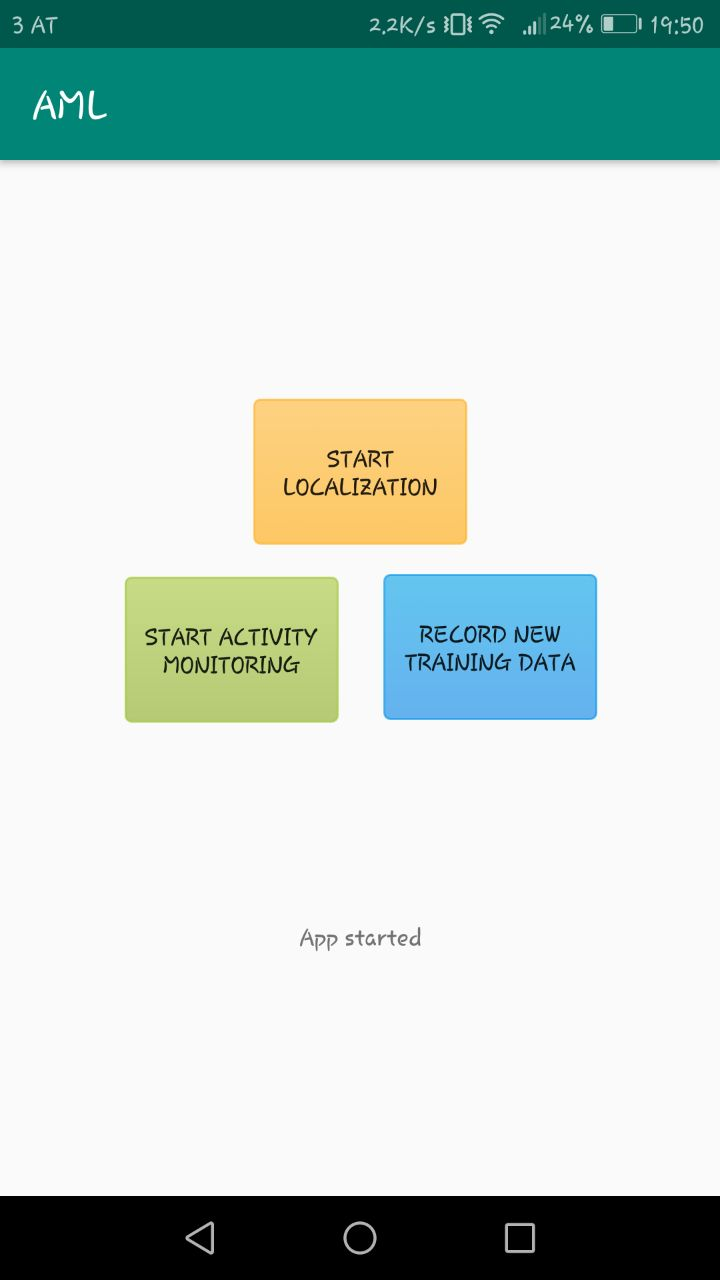
\includegraphics[width=140px]{images/main.jpeg}
	\caption{Home screen}
	\label{fig:main}
\end{figure}

\subsection{Activity Monitoring}
The Activity Monitoring is split into two activities, one collects training data and stores it into a file locally. The other activity monitors the sensors and uses the kNN algorithm to classify the user's motion.

\subsubsection{Background: Activity monitoring using KNN}

\subsubsection{Train Activity} \label{sec:train}
This activity enables the user to collect training data for the monitoring activity. 1 of 4 activities are currently implemented, however any activity can be trained, only the label would mismatch at the moment.
\\
The user needs to press one of the activities and perform the motion. The accelerometer data is sampled over a predefined window and the timestamp, mean of the x, y and z axis as well as the minimum and maximum of the euclidean distance is stores in a local .txt file. The most dominant frequency is also stored but it is currently not used as it lowers the recognition accuracy.
\\
If a faulty measurement was recorded the user can delete the last entry or delete the whole .txt file.

\begin{center}
  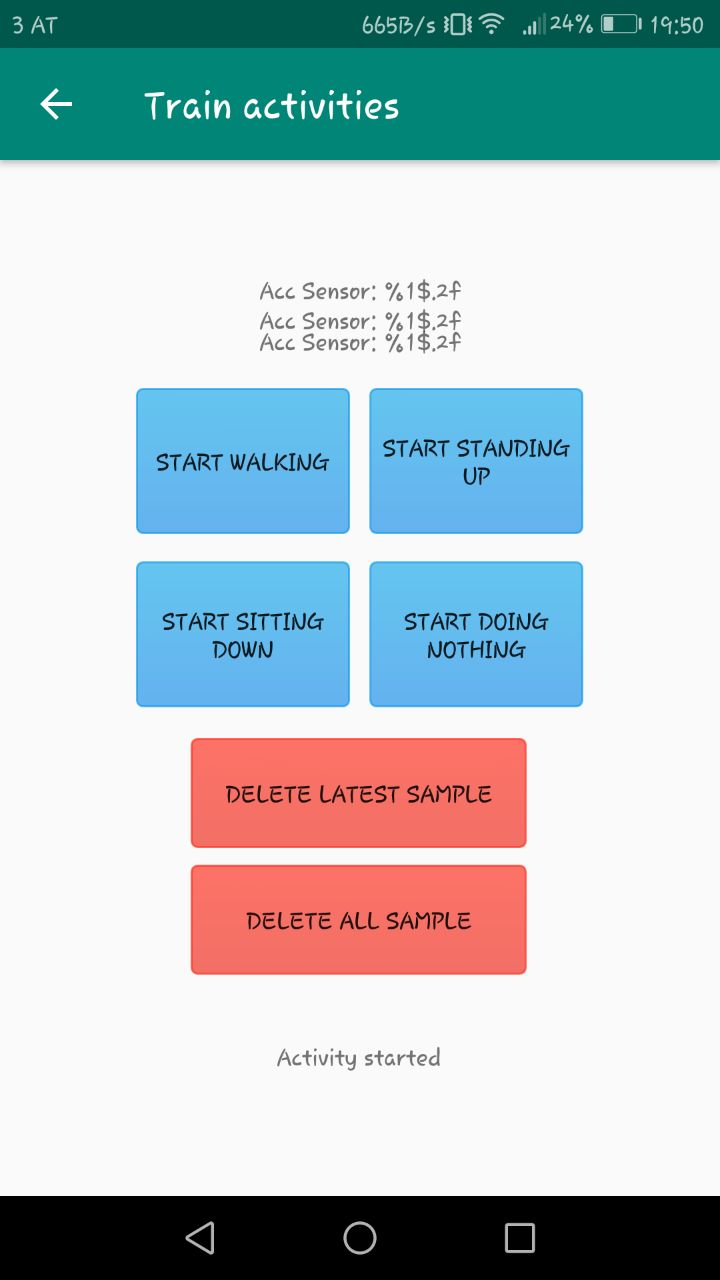
\includegraphics[width=140px]{images/train_activity}
\end{center}

\pagebreak
 
\subsubsection{Monitoring} \label{sec:monitoring}


The second activity tries to classify the activity currently performed by the user. When the button is pressed, the accelerometer data is sampled with the same window size as the training data. 
\\
Then a kNN algorithm finds the nearest neighbours by calculating the euclidean distance of the averaged coordinates to each training record and selecting the k closest ones. 
\\
Then we classify the neighbours by weighting each label and adding the weights if a label occurs more than once. This gives us a probability of how certain we are of our match. The recognized activity is displayed together with the probabilities for each of our 4 predefined activities.
\\
When the "continuous monitoring" box is ticked, this prediction process (sample, kNN, classify) is repeated endlessly.

\begin{center}
  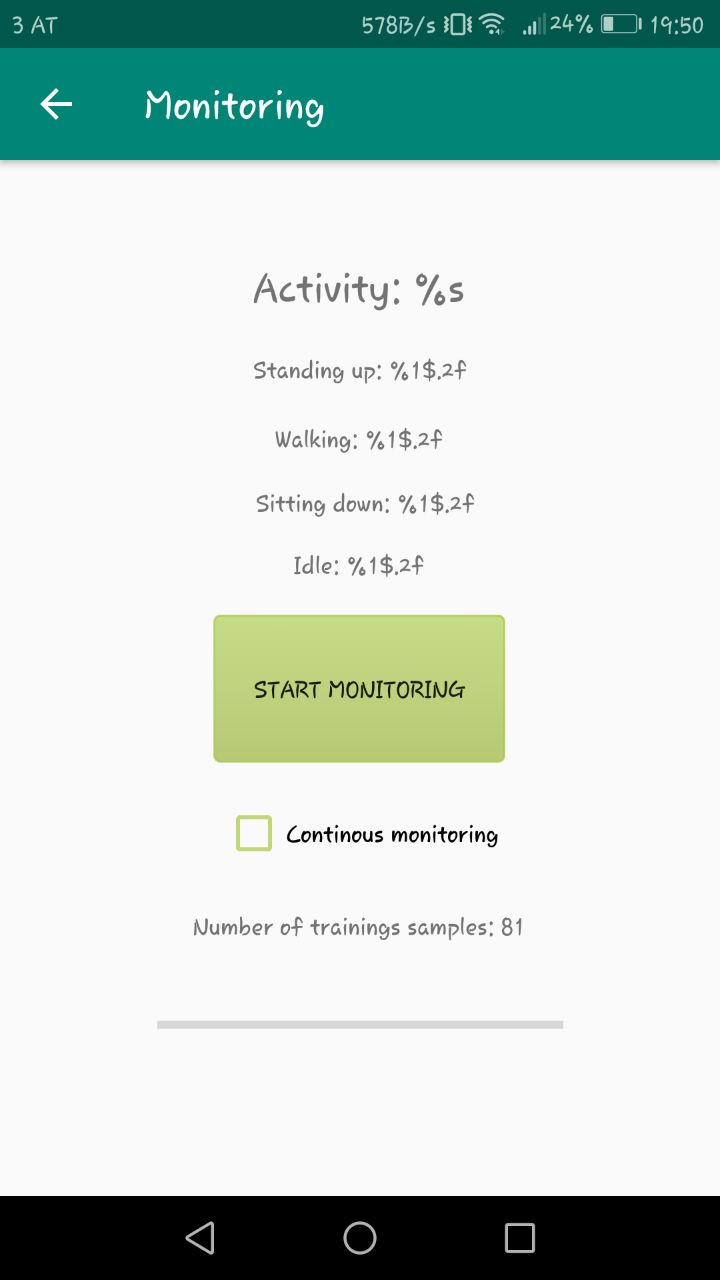
\includegraphics[width=140px]{images/monitoring.jpeg}
\end{center}

\pagebreak

\subsubsection{Limitation/Challenges}

%Python script, accuracy etc.

\subsection{Localization} \label{sec:localization}

\subsubsection{Background: Particle Filter}





\subsubsection{Implementation}
\subsubsection*{GUI}
As shown in Figure \ref{fig:localization}, the localization activity displays a map of the ITI building's first floor, text fields to report the users movement, an arrow indicating the user's current orientation and three buttons to 
\begin{itemize}[noitemsep,topsep=0pt]
	\item move a single particle
	\item init particles and start localization
	\item show the walls of the building on the map (mainly debug purposes)
\end{itemize}

\begin{figure}
	\centering
	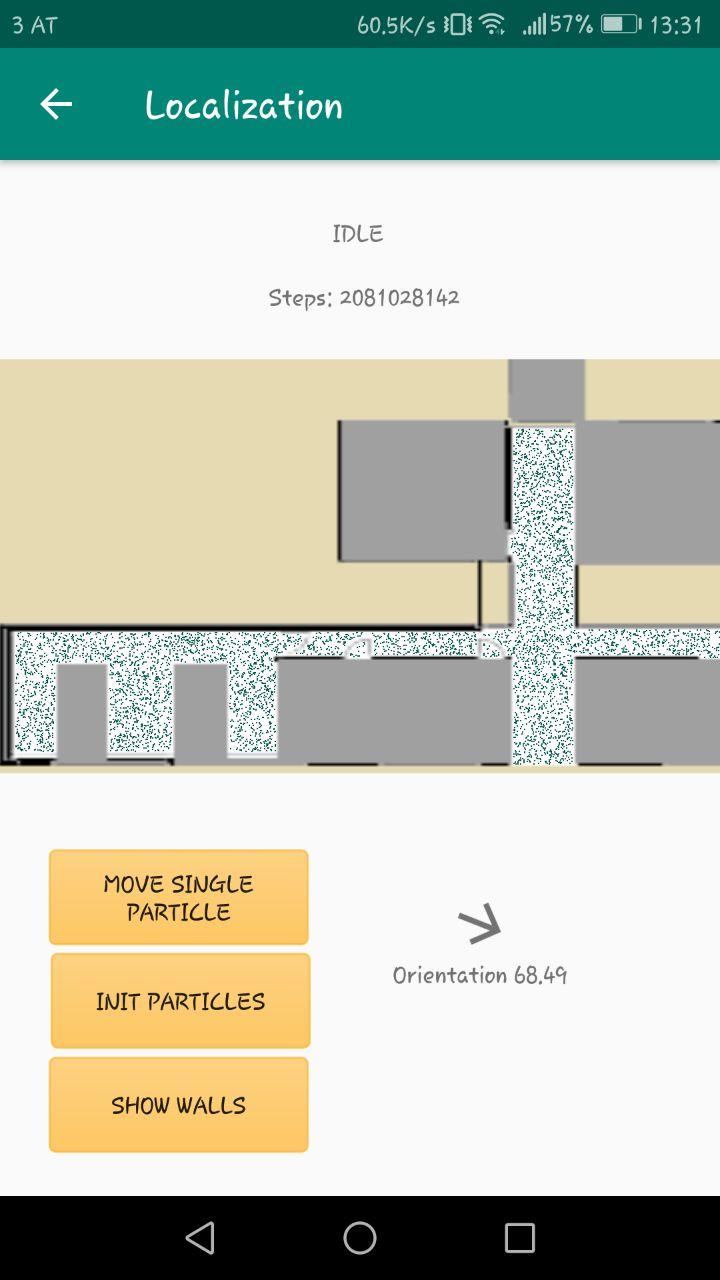
\includegraphics[width=140px]{images/localization.jpeg}
	\caption{UI of localization activity}
	\label{fig:localization}
\end{figure}

\subsubsection*{Movement detection}
In order to detect the user's movement to create an appropriate movement model, we utilized the smartphone's build in accelerometer and magnetic sensor. The movement detection is implemented in a background service.

The user's orientation is retrieved using the Android method \textit{getOrientation}. Since the value is quite inaccurate, the median value of the measurement while walking is used.

To detect if the user started respectively stopped walking, the %TODOO: explain and cite reference (olga's page)

\subsubsection*{Particle Filter parameterization}


\subsubsection{Limitations/Challenges}
The main challenge was the inaccuracy of the orienatation measurements. During the debugging process, we 
\bibliographystyle{ieeetr}
\bibliography{refs}



\end{document}